% omega-paper-2.tex --
%%%%%%%%%%%%%%%%%%%%%%%%%%%%%%%%%%%%%%%%%%%%%%%%%%%%%%%%%%%%%%%%%%%%%%%%
\NeedsTeXFormat{LaTeX2e}
\documentclass[12pt,a4paper]{article}
\usepackage{type1cm}
\usepackage{graphicx,feynmp,emp}
\DeclareGraphicsRule{*}{mps}{*}{}
\usepackage{verbatim,array,amsmath,amssymb,amscd,url}
\usepackage{thophys}
\usepackage{thohacks}
\setlength{\unitlength}{1mm}
\empaddtoTeX{\usepackage{amsmath,amssymb}}
\empaddtoTeX{\usepackage{thophys,thohacks}}
\empaddtoprelude{input graph;}
\empaddtoprelude{input boxes;}
%%%%%%%%%%%%%%%%%%%%%%%%%%%%%%%%%%%%%%%%%%%%%%%%%%%%%%%%%%%%%%%%%%%%%%%%
\widowpenalty=4000
\clubpenalty=4000
\displaywidowpenalty=4000
\allowdisplaybreaks
\renewcommand{\topfraction}{0.9}
\renewcommand{\bottomfraction}{0.9}
\renewcommand{\textfraction}{0.1}
\setlength{\abovecaptionskip}{.5\baselineskip}
\setlength{\belowcaptionskip}{\baselineskip}
%%%%%%%%%%%%%%%%%%%%%%%%%%%%%%%%%%%%%%%%%%%%%%%%%%%%%%%%%%%%%%%%%%%%%%%%
\newenvironment{code}{\verbatim}{\endverbatim\noindent}
\DeclareMathOperator{\tr}{tr}
\newcommand{\dd}{\mathrm{d}}
\newcommand{\ii}{\mathrm{i}}
\newcommand{\ee}{\mathrm{e}}
\renewcommand{\Re}{\text{Re}}
\renewcommand{\Im}{\text{Im}}
\newcommand{\ketbra}[2]{\ket{#1}\!\bra{#2}}
\newcommand{\Ketbra}[2]{\Ket{#1}\!\Bra{#2}}
\def\OCaml/{\texttt{ocaml}}
%%%%%%%%%%%%%%%%%%%%%%%%%%%%%%%%%%%%%%%%%%%%%%%%%%%%%%%%%%%%%%%%%%%%%%%%
\newcommand{\eprint}[1]{\ahref{http://arXiv.org/abs/#1}{#1}}
\def\OMEGA/{\texttt{O'Mega}}
%%%%%%%%%%%%%%%%%%%%%%%%%%%%%%%%%%%%%%%%%%%%%%%%%%%%%%%%%%%%%%%%%%%%%%%%
\begin{document}
\begin{fmffile}{\jobname pics}
\fmfset{arrow_ang}{10}
\fmfset{curly_len}{2mm}
\fmfset{wiggly_len}{3mm}
\begin{empfile}
%%%%%%%%%%%%%%%%%%%%%%%%%%%%%%%%%%%%%%%%%%%%%%%%%%%%%%%%%%%%%%%%%%%%%%%%
%%%%%%%%%%%%%%%%%%%%%%%%%%%%%%%%%%%%%%%%%%%%%%%%%%%%%%%%%%%%%%%%%%%%%%%%
\title{%
  O'Mega:\\An~Optimizing~Matrix~Element~Generator.\\
  II: Amplitudes~With~Color~Flow and Without~Fermion~Number~Conservation}
\author{%
  Wolfgang Kilian\thanks{\texttt{kilian@hep.physik.uni-siegen.de}}\\
  \hfil\\
    Theoretische Physik 1\\
    Universit\"at Siegen\\
    Walter-Flex-Str.~3, 57068 Siegen, Germany\\ 
  \hfil\\
  Thorsten Ohl\thanks{\texttt{ohl@physik.uni-wuerzburg.de},
    \texttt{http://physik.uni-wuerzburg.de/ohl}}\\
  \hfil\\
    Institut f\"ur Theoretische~Physik und Astrophysik\\
    Universit\"at~W\"urzburg\\
    Emil-Hilb-Weg 22, 97074~W\"urzburg, Germany\\
  \hfil\\
  J\"urgen Reuter\thanks{\texttt{juergen.reuter@desy.de}}\\
  \hfil\\
   Deutsches Elektronen-Synchrotron DESY\\
   Notkestra\ss{}e 85, 22607 Hamburg, Germany}
\date{%
  \fbox{\qquad DESY 11-131 \qquad}\\
  \hfil\\
\today}
\maketitle
\newpage
\begin{abstract}
  This paper describes features of the optimizing matrix element generator 
  O'Mega that have been implemented since it was first made publically
  available about 10~years ago.  The outstanding additions are an efficient
  intrinsic implementation of color flow amplitudes and support for
  Fermi statistics without conserved fermion number.
\end{abstract}
%%%%%%%%%%%%%%%%%%%%%%%%%%%%%%%%%%%%%%%%%%%%%%%%%%%%%%%%%%%%%%%%%%%%%%%%
\section{Introduction}
\label{sec:intro}

This paper is a companion to~\cite{Moretti:2001zz}, which is a
minimally updated version of the preprint that was circulated first when O'Mega
became public 10 years ago.  It will henceforth be referred to as~I.

\begin{dubious}
The standard intro stuff \ldots
\end{dubious}

%%%%%%%%%%%%%%%%%%%%%%%%%%%%%%%%%%%%%%%%%%%%%%%%%%%%%%%%%%%%%%%%%%%%%%%%
\section{Color Flow Amplitudes}
\label{sec:color}

When O'Mega was first developed in the context of studies for a
$e^+e^-$ linear collider, the color degrees of freedom could be taken
into account trivially for many interesting processes.  Also it was
not yet clear, which external and internal representations
would produce the most efficient
und useful results for practical use in Monte Carlo simulations of
processes with many colored particles, e.\,g.~at LHC.

Later, version~1 of WHIZARD~\cite{Kilian:2007gr} employed this version
of O'Mega with 
Feynman rules for particles with an explicit color flow quantum
number~\cite{Maltoni:2002mq} to compute
full scattering amplitudes for colored particles, including all
interferences.  This approach proved to very fruitful, since the
resulting code is both numerically efficient and contains, in contrast
to analytically color summed amplitudes, all the information required
for parton showers and hadronization.

Nevertheless, this approach suffered from two major drawbacks: firstly
the implementation of Feynman rules in the color flow basis is a
tedious, repetitive and thererfore error prone task, in particular in
models with many particles and vertices, such as supersymmetric
extensions of the standard model.  Secondly, while the final code is
numerically very efficient, its generation consumed a lot of memory
and time.  The former was caused by an explosion in the number of
particles and vertices and the corresponding lookup tables since each
particle must be duplicated for all possible color flows.  The
resulting memory accesses slowed the program down, together with the
dramatically increased number of combinations that had to be tried
when building the DAG -- most of which would not contribute to the
final result.

Both problems were addressed successfully by handling color in O'Mega
explicitely and not as just another quantum number.

%%%%%%%%%%%%%%%%%%%%%%%%%%%%%%%%%%%%%%%%%%%%%%%%%%%%%%%%%%%%%%%%%%%%%%%%
\subsection{The \texttt{Colorize} Functor}
\label{sec:colorize-models}

As mentioned above, deriving the Fenman rules in the color flow basis
is a repetitive task. It is therefore perfectly suited for
implementation in a computer program.  Each \OMEGA/ model is represented
by an \OCaml/ module with functions that are used to inquire the
available particles, their quantum numbers and the ways in which they
couple at the vertices.  Thus a functor \texttt{Colorize} can be
implemented, that maps a module representing a model with given color
representations to a new module representing a new model with Feynman
rules in the color flow 
representation.  As long as all matter fields live in the
fundamental representation or its conjugate, there are only
renormalizable couplings and there are no
$\epsilon_{ijk}$-style couplings, the Feynman rules for the color
flows can be inferred
from the representations alone.  In the general case~\cite{cflow}, which
will be implemented later, additional annotation will be required.


%%%%%%%%%%%%%%%%%%%%%%%%%%%%%%%%%%%%%%%%%%%%%%%%%%%%%%%%%%%%%%%%%%%%%%%%
\subsection{Adding color to amplitudes}
\label{sec:colorize-amplitudes}

%%%%%%%%%%%%%%%%%%%%%%%%%%%%%%%%%%%%%%%%%%%%%%%%%%%%%%%%%%%%%%%%%%%%%%%%
\section{The Great Line-up: Fermion-number violating vertices}
\label{sec:majo}

\subsection{The problem}

The determination of the relative sign of different parts of an
S-matrix element or quantum field-theoretical amplitude due to the
sign changes from anticommuting fermion fields according to Wick's
theorem has been described in the first
paper~\cite{Moretti:2001zz}. However, such an approach is strictly
only applicable to completely vector-like theories like QED or QCD
with gauge fields and matter fields that only interact via gauge
interactions. As soon as matter interactions via Yukawa-type couplings
are involved, it crucially depends on the content of matter
representations whether such a description based on the conservation
of fermion number is sufficient or not. In the Standard Model, there
are accidentally only couplings which respect fermion number because
of the strong constraints from the quantum numbers. In principle, it
is the non-existence of a scalar particle carrying either lepton or
color quantum numbers which disallows fermion-number violating
vertices at the renormalizable level. Consider the case of a charge
-1/3 scalar particle in the fundamental color representation, which
could couple together with an up-type and down-type quark to a
singlet. This interaction term (which appears e.g. in $R$-parity
violating supersymmetry) has to be described by one of the following
two vertices: 
\begin{equation*}
          \begin{fmfgraph*}(20,15)
                \fmfstraight
                \fmfleft{l1,l2}         
                \fmfright{r}
                \fmf{fermion,label=$\Psi$,l.side=left}{l2,c}
                \fmf{fermion,label=$\Psi$,l.side=left}{l1,c}
                \fmf{dashes}{c,r}
                \fmf{dots}{c}    
          \end{fmfgraph*}
          \qquad
          \begin{fmfgraph*}(20,15)
                \fmfstraight
                \fmfleft{l1,l2}         
               \fmfright{r}
                \fmf{fermion,label=$\overline\Psi$,l.side=right}{c,l2}
                \fmf{fermion,label=$\overline\Psi$,l.side=right}{c,l1}
                \fmf{dashes}{c,r}
                \fmf{dots}{c}    
          \end{fmfgraph*}
\end{equation*}
These vertices are historically known as ``clashing-arrow''
vertices. Note that one could try to revert one of the arrows by using
a charge-conjugation matrix, which converts a spinor into its
charge-conjugated spinor. Such Feynman rules always contain an
explicit charge-conjugation matrix and can e.g. be found
in~\cite{Haber:1984rc}. But they are quite error-prone when using them
in operations like crossing, and the explicit presence of the
charge-conjugation matrix makes the determination of the relative
signs between different parts of amplitudes cumbersome. 

A different kind of vertices appears with the presence of neutral
fermions which could be described by a four-component bispinor with
left- and right-handed components related by complex conjugation,
known as a Majorana spinor. Note that such a particle does not need to
be completely uncharged, but could be in a real representation of a 
non-Abelian symmetry like the gluino in supersymmetry. Sometimes,
Majorana fermions are denoted by lines with arrows pointing in both
directions, especially in the context of Majorana mass terms, thereby
denoting the fact that a Majorana mass term does {\em not} change
chirality, but is vector-like. We consider Majorana fermions to be
characterized as being there own antiparticles, and hence denote them
by a line without any arrow. This leads to vertices of the type:
\begin{equation*}
          \begin{fmfgraph*}(20,15)
                \fmfstraight
                \fmfleft{l1,l2}         
                \fmfright{r}
                \fmf{plain,label=$\chi$,l.side=left}{l2,c}
                \fmf{plain,label=$\chi$,l.side=left}{l1,c}
                \fmf{dashes}{c,r}
                \fmf{dots}{c}    
          \end{fmfgraph*}
          \qquad
          \begin{fmfgraph*}(20,15)
                \fmfstraight
                \fmfleft{l1,l2}         
               \fmfright{r}
                \fmf{plain,label=$\chi$,l.side=right}{c,l2}
                \fmf{fermion,label=$\Psi$,l.side=right}{l1,c}
                \fmf{dashes}{c,r}
                \fmf{dots}{c}    
          \end{fmfgraph*}
          \qquad
          \begin{fmfgraph*}(20,15)
                \fmfstraight
                \fmfleft{l1,l2}         
                \fmfright{r}
                \fmf{fermion,label=$\overline\Psi$,l.side=right}{c,l1}
                \fmf{plain,label=$\chi$,l.side=right}{c,l2}
                \fmf{dashes}{c,r}
                \fmf{dots}{c}    
          \end{fmfgraph*}
          \qquad
          \begin{fmfgraph*}(20,15)
                \fmfstraight
                \fmfleft{l1,l2}         
                \fmfright{r}
                \fmf{plain,label=$\chi$,l.side=right}{c,l2}
                \fmf{plain,label=$\chi$,l.side=right}{c,l1}
                \fmf{gluon}{c,r}
                \fmf{dots}{c}    
          \end{fmfgraph*}
\end{equation*}

Consistent Feynman rules for fermion-number violating vertices,
including both clashing arrows and Majorana fermions, have been constructed
in~\cite{Denner:1992vza}. 

\subsection{The solution and algorithm}

To summarize, there are now six types of vertices involving fermions:
\begin{align}
        \parbox{17mm}{\hfil\\
        \begin{fmfgraph*}(15,12)
                \fmftop{t}
                \fmfbottom{b1,b2}
                \fmf{fermion}{b2,v,b1}
                \fmf{dashes}{v,t}
                \fmfdot{v}
        \end{fmfgraph*}\hfil\\}  \quad
        \parbox{17mm}{\hfil\\
        \begin{fmfgraph*}(15,12)
                \fmftop{t}
                \fmfbottom{b1,b2}
                \fmf{fermion}{b2,v}
                \fmf{plain}{v,b1}
                \fmf{dashes}{v,t}
                \fmfdot{v}
        \end{fmfgraph*}\hfil\\}  \quad
        \parbox{17mm}{\hfil\\
        \begin{fmfgraph*}(15,12)
                \fmftop{t}
                \fmfbottom{b1,b2}
                \fmf{fermion}{v,b1}
                \fmf{plain}{v,b2}
                \fmfdot{v}
                \fmf{dashes}{v,t}
        \end{fmfgraph*}\hfil\\}  \quad
        \parbox{17mm}{\hfil\\
        \begin{fmfgraph*}(15,12)
                \fmftop{t}
                \fmfbottom{b1,b2}
                \fmf{plain}{b2,v,b1}
                \fmf{dashes}{v,t}
                \fmfdot{v}
        \end{fmfgraph*}\hfil\\}  \quad
        \parbox{17mm}{\hfil\\
        \begin{fmfgraph*}(15,12)
                \fmftop{t}
                \fmfbottom{b1,b2}
                \fmf{fermion}{b2,v}
                \fmf{fermion}{b1,v}
                \fmf{dashes}{v,t}
                \fmfdot{v}
        \end{fmfgraph*}\hfil\\}  \quad  
        \parbox{17mm}{\hfil\\
        \begin{fmfgraph*}(15,12)
                \fmftop{t}
                \fmfbottom{b1,b2}
                \fmf{fermion}{v,b1}
                \fmf{fermion}{v,b2}
                \fmf{dashes}{v,t}
                \fmfdot{v}
        \end{fmfgraph*}\hfil\\}
\end{align}
The dashed line indicates an arbitrary boson. Note that the Majorana
fermion is not restricted to be a spin 1/2-particle, but could also be
a spin 3/2 gravitino, wich couples to a spin 1/2 fermion and a vector.
Since there is no longer a well-defined direction along the fermion lines
(there may be parts of lines having no direction at all due to propagating
Majorana fermions, or the line's direction changes by one of the rightmost 
vertices) the method presented in~\cite{Moretti:2001zz} is no longer
feasible. One possibility is to artificially assign a direction to a
Majorana line and define different vertices for each case in which the
arrows direct to or from the vertex~\cite{Haber:1984rc}. This
would give the correct analytical expressions for the Feynman
diagrams, but the signs between different diagrams contributing to 
the same amplitude have to be derived by means of Wick's theorem,
which is no good solution for implementing such rules in a computer
program. Instead we follow the rather generic approach
of~\cite{Denner:1992vza}. The concept of {\em fermion number
  conservation} is abandoned, and we only use the assumption of 
{\em fermion conservation} which is the fact that half-integer Lorentz
representations can only be generated or destroyed in pairs (and
fermion lines must run uninterrupted through diagrams).
The disentanglement of vertex operators to calculate relative signs by
Wick's theorem is done by the standard external states for bispinors,
propagators and vertices as well as their charge-conjugated versions: 
\begin{subequations}
\label{eq:cc_rules}
\begin{align}
  \mathcal{C} \overline{v}^T_\sigma (p) &=\; u_\sigma (p) \\
  \mathcal{C} \overline{u}^T_\sigma (p) &=\; v_\sigma (p) \\
  S'_F \equiv \mathcal{C} S_F^T (p) \mathcal{C}^{-1}  &=\; S_F (-p) =
  \dfrac{\ii}{-\fmslash{p} - m}  
  \label{eq:propprime} 
  \\
  \Gamma' \equiv \mathcal{C} \Gamma^T \mathcal{C}^{-1} &=\; \left\{ 
    \begin{array}{ll}
      + \Gamma & \quad \text{for} \;\; \Gamma \equiv \mathbb{I}, \gamma^5
      \gamma^\mu, \gamma^\mu \\ 
      - \Gamma & \quad \text{for} \;\; \Gamma \equiv \gamma^\mu,
      \sigma^{\mu\nu} 
    \end{array} \right. , \label{eq:gammagammastrich} 
\end{align}
\end{subequations}
where $\mathcal{C}$ is the charge conjugation matrix. 

The basic idea for disentangling contractions of fermionic field
operators in any non-standard ordering (for more details
cf.~\cite{Denner:1992vza}) is to replace an interaction term bilinear
in fermionic field operators by its transpose:
$\overline{\Psi}\Gamma\Psi = \left( \overline{\Psi} \Gamma
\Psi \right)^T$. This does not change anything as this operator is
just a complex number. Performing the transposition and replacing
operators and gamma matrices by their charge-conjugated versions, 
\begin{equation}
        \label{eq:entangle}
  \contracted{}{\stackrel{\stackrel{\hfil}{\hfil}}{\ldots}}{\;}
  {\contracted{}{\overline{\Psi}}{\Gamma\Psi\;\;\:}{\ldots}}{} 
  \qquad \longrightarrow \qquad (-1) \cdot
  \contracted{}{\stackrel{\stackrel{\hfil}{\hfil}}{\ldots}}{}{\Psi^T\:}
  \mathcal{C}^{-1} \left(\mathcal{C} \Gamma^T \mathcal{C}^{-1} \right)
  \mathcal{C} \contracted{}{\;\;\overline{\Psi}^T}{}{\ldots} 
  \quad ,
\end{equation}
disentangles the contraction on the left-hand side. The sign comes
from anticommuting the field operators. Such entangled contractions
can in fact appear as for Majorana fermions all four contractions
between field operators and their conjugates are non-vanishing, and
also due to the appearance of explicitly charged conjugated fermions
as e.g. in a chargino--fermion--sfermion vertex. Note that for
(explicitly charged) Dirac fermions such contractions only happen in
two cases: i) for the contraction of the creation and annihilation
operators inside field operators with the asymptotic external states,
which produces a global sign which is irrelevant (but becomes crucial
when comparing different $S$-matrix elements in Slavnov-Taylor
identities), and ii) in a closed fermion loop. 

The analytical expression for a complete fermion line is just a
sandwich of mutual products of vertex factors and propagators between
two external bispinor states. Transposing such a complete fermion line
using the expressions in Eqs.~(\ref{eq:cc_rules}) yields
($w \in \left\{ u, v \right\}$, $w^c \in \left\{ u^c = v, v^c = u
\right\}$ with $w^c \equiv \mathcal{C} \overline{w}^T$):
\begin{equation}
        \label{eq:entangle2}
        \overline{w}_1 \Gamma^{(1)} S_F^{(1)} \Gamma^{(2)} \ldots
        \Gamma^{(n)} w_2 = (-1) \cdot \overline{w^c_2} \, 
        \Gamma^{\prime\,(n)} \ldots S_F^{\prime\,(1)} \Gamma^{\prime\,
        (1)} w^c_1 , 
\end{equation}
Note that such an analytical expression does not contain any
anticommuting objects any more. Hence, the sign does not come from
fermion anticommutation but from the antisymmetry of the charge
conjugation matrix: $w^T = \overline{w^c} \, \mathcal{C}^T = -
\overline{w^c} \, \mathcal{C}$. 

Both ways of evaluating a fermion line produce the same result as the
sign in Eq.~(\ref{eq:entangle2}) is cancelled by the one from fermion 
anticommutation in Eq.~(\ref{eq:entangle}). Hence, it does not matter in
which way to evaluate a fermion line, as
conjugated spinors can always be transferred via transposition into
spinors and vice versa. So the key ingredient of the rules
in~\cite{Denner:1992vza} is to just choose arbitrarily a direction to
evaluate a fermion line, which is no longer determined by where there
is the conjugated spinor and where the spinor as for a theory with
purely Dirac spinors and non-clashing arrow vertices only. Whenever
the arbitrarily chosen evaluation direction is opposite to the fermion
arrow, one writes down the charge-conjugated (primed) expressions
from Eq.~(\ref{eq:cc_rules}). Thereby, the disentanglement of fermionic
contractions is automatically guaranteed, and there is no need to
explicitly use Wick's theorem. The relative signs of different diagrams
can then be evaluated by the same method of permutations of pairs of
external fermions connected by lines with respect to a reference order
as in~\cite{Moretti:2001zz}. However, now the fermion pairs are not of
the form \verb+(conjugated spinor, spinor)+, but simply
\verb+(endpoint, starting point)+ of the corresponding fermion line.
For more technical details cf.~\cite{Denner:1992vza,Reuter:2002gn}.

\subsection{The implementation}


\begin{figure}
\[
     \setlength{\extrarowheight}{2pt}     
     \setlength{\fboxsep}{3mm}
        \begin{array}{cccc}
        \text{Fermion} & \;\;\;\text{Antifermion} & \;\;\text{Majorana
     fermion} & \text{Assignment} \\ & & & \\ 
          \parbox{18mm}{\hfil\\        
        \begin{fmfgraph*}(17,5)
          \fmfleft{l1,l2}
          \fmfright{r1,r2}
          \fmfbottomn{b}{8}
          \fmf{fermion}{l2,r2}
          \fmf{dots}{b2,b6}
          \fmf{phantom_arrow}{b6,b7}
          \fmfv{decor.shape=circle,decor.filled=30,
                         decor.size=3mm}{l2}  
        \end{fmfgraph*}} &  \qquad \parbox{18mm}{\hfil\\
        \begin{fmfgraph*}(17,5)
          \fmfleft{l1,l2}
          \fmfright{r1,r2}
          \fmfbottomn{b}{8}
          \fmf{fermion}{r2,l2}
          \fmf{dots}{b2,b6}
          \fmf{phantom_arrow}{b6,b7}
          \fmfv{decor.shape=circle,decor.filled=30,
                         decor.size=3mm}{l2}  
        \end{fmfgraph*}}        &  \qquad \parbox{18mm}{\hfil\\
        \begin{fmfgraph*}(17,5)
          \fmfleft{l1,l2}
          \fmfright{r1,r2}
          \fmfbottomn{b}{8}
          \fmf{plain}{l2,r2}
          \fmf{dots}{b2,b6}
          \fmf{phantom_arrow}{b6,b7}
          \fmfv{decor.shape=circle,decor.filled=30,
                         decor.size=3mm}{l2}  
        \end{fmfgraph*}}        & \qquad\overline{u}_\sigma (p) \\ & & & \\  
          \framebox{\parbox{18mm}{\hfil\\              
        \begin{fmfgraph*}(17,5)
          \fmfleft{l1,l2}
          \fmfright{r1,r2}
          \fmfbottomn{b}{8}
          \fmf{fermion}{l2,r2}
          \fmf{dots}{b3,b7}
          \fmf{phantom_arrow}{b3,b2}
          \fmfv{decor.shape=circle,decor.filled=30,
                         decor.size=3mm}{l2}  
        \end{fmfgraph*}}} &  \qquad \framebox{\parbox{18mm}{\hfil\\
        \begin{fmfgraph*}(17,5)
          \fmfleft{l1,l2}
          \fmfright{r1,r2}
          \fmfbottomn{b}{8}
          \fmf{fermion}{r2,l2}
          \fmf{dots}{b3,b7}
          \fmf{phantom_arrow}{b3,b2}
          \fmfv{decor.shape=circle,decor.filled=30,
                         decor.size=3mm}{l2}  
        \end{fmfgraph*}}}       &  \qquad \framebox{\parbox{18mm}{\hfil\\
        \begin{fmfgraph*}(17,5)
          \fmfleft{l1,l2}
          \fmfright{r1,r2}
          \fmfbottomn{b}{8}
          \fmf{plain}{l2,r2}
          \fmf{dots}{b3,b7}
          \fmf{phantom_arrow}{b3,b2}
          \fmfv{decor.shape=circle,decor.filled=30,
                         decor.size=3mm}{l2}  
        \end{fmfgraph*}}}       & \qquad v_\sigma(p) \\ & & & \\ 
          \framebox{\parbox{18mm}{\hfil\\              
        \begin{fmfgraph*}(17,5)
          \fmfleft{l1,l2}
          \fmfright{r1,r2}
          \fmfbottomn{b}{8}
          \fmf{fermion}{l2,r2}
          \fmf{dots}{b2,b6}
          \fmf{phantom_arrow}{b6,b7}
          \fmfv{decor.shape=circle,decor.filled=30,
                         decor.size=3mm}{r2}  
        \end{fmfgraph*}}} &  \qquad \framebox{\parbox{18mm}{\hfil\\
        \begin{fmfgraph*}(17,5)
          \fmfleft{l1,l2}
          \fmfright{r1,r2}
          \fmfbottomn{b}{8}
          \fmf{fermion}{r2,l2}
          \fmf{dots}{b2,b6}
          \fmf{phantom_arrow}{b6,b7}
          \fmfv{decor.shape=circle,decor.filled=30,
                         decor.size=3mm}{r2}  
        \end{fmfgraph*}}}       &  \qquad \framebox{\parbox{18mm}{\hfil\\
        \begin{fmfgraph*}(17,5)
          \fmfleft{l1,l2}
          \fmfright{r1,r2}
          \fmfbottomn{b}{8}
          \fmf{plain}{l2,r2}
          \fmf{dots}{b2,b6}
          \fmf{phantom_arrow}{b6,b7}
          \fmfv{decor.shape=circle,decor.filled=30,
                         decor.size=3mm}{r2}  
        \end{fmfgraph*}}}       & \qquad u_\sigma (p) \\ & & & \\ 
          \parbox{18mm}{\hfil\\        
        \begin{fmfgraph*}(17,5)
          \fmfleft{l1,l2}
          \fmfright{r1,r2}
          \fmfbottomn{b}{8}
          \fmf{fermion}{l2,r2}
          \fmf{dots}{b3,b7}
          \fmf{phantom_arrow}{b3,b2}
          \fmfv{decor.shape=circle,decor.filled=30,
                         decor.size=3mm}{r2}  
        \end{fmfgraph*}} &  \qquad \parbox{18mm}{\hfil\\
        \begin{fmfgraph*}(17,5)
          \fmfleft{l1,l2}
          \fmfright{r1,r2}
          \fmfbottomn{b}{8}
          \fmf{fermion}{r2,l2}
          \fmf{dots}{b3,b7}
          \fmf{phantom_arrow}{b3,b2}
          \fmfv{decor.shape=circle,decor.filled=30,
                         decor.size=3mm}{r2}  
        \end{fmfgraph*}}        &  \qquad \parbox{18mm}{\hfil\\
        \begin{fmfgraph*}(17,5)
          \fmfleft{l1,l2}
          \fmfright{r1,r2}
          \fmfbottomn{b}{8}
          \fmf{plain}{l2,r2}
          \fmf{dots}{b3,b7}
          \fmf{phantom_arrow}{b3,b2}
          \fmfv{decor.shape=circle,decor.filled=30,
                         decor.size=3mm}{r2}  
        \end{fmfgraph*}}        & \qquad \overline{v}_\sigma (p)
        \end{array} \]
\caption{\label{fig:rules_ext} 
 Feynman rules for external fermions for theories with fermion-number
 violating vertices. Evaluation directions are denoted by dotted
 arrows. The time flow is from left to right. According to the
 implementation in O'Mega using an inward pointing evaluation
 direction only the rules inside the boxes are used.} 
\end{figure}

Now, after it is clear how to determine relative signs and calculate
expressions for fermion-number violating vertices, this algorithm has
to be implemented in a compatible way into O'Mega. The difficulty is
that there are no complete Feynman diagrams present, but only
subamplitudes representing 1POWs. The simple solution is to just
assign an inward pointing evaluation direction for external fermions
and to follow open lines keeping that evaluation direction until they
are fused with a second line (either to yield a bosonic 1POW or a
complete amplitude in a final \verb+keystone+). Hence, external
particles are always assigned a bispinor (i.e. $u$ or $v$), but never
a conjugated bispinor, $\overline{u}$ or
$\overline{v}$. Fig.~\ref{fig:rules_ext} summarizes the Feynman rules
of~\cite{Denner:1992vza} for external fermions, where the grey blob
signifies the residual amplitude. As pointed out above, the evaluation
direction is chosen such that it always points from the external
fermion inward into the rest of the amplitude. Hence, only the cases
inside the boxes are used, i.e. we never assign conjugated spinors to
external fermions. In detail, incoming (with respect to the time axis)
fermions, antifermions and Majorana fermions are always assigned a $u$
spinor, while the corresponding outgoing particles are denoted by a
$v$ spinor. 

Consequently, in the implementation of the Feynman rules for
fermions with fermion-number violating vertices, no conjugated spinors
appear at all. External spinors $u$ and $v$ get left-multiplied by
gamma matrices from vertices as well as from propagators, yielding
again a spinor, and not a conjugated spinor. Finally, when two lines
are fused into a closed fermion line (not in the sense of a loop, but
running from one external fermion to another), we simply have to use
the bilinear product $\Psi^T_1 \mathcal{C} \Gamma \Psi_2$ between two 
spinors (containing an explicit charge-conjugation matrix), instead of
the ordinary bilinear product, $\overline{\Psi}_1 \Gamma
\Psi_2$ between a conjugated spinor and a spinor. 

This bilinear product takes into account the fact, that when closing
two open fermion lines in a final fusion, the evaluation direction of
one of the two lines has to be reverted. This means, that finally a 
unique evaluation direction for the complete fermion line is chosen
as soon as after the final fusion the complete course of the fermion
line within the subamplitude is known. There are two choices, to
revert either the fermion line from the left leg or the right leg of
the fusion: 
\begin{equation}
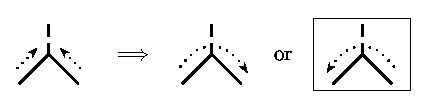
\includegraphics[width=.4\paperwidth]{mom_choice}
\end{equation}
So when closing a fermion line in a fusion, we finally choose the
evaluation direction to go from the end of the right leg through the
fusion to the external end of the left leg, thereby reverting the
original evaluation direction of the left leg. In principle, one would
have to take a conjugated spinor $\overline{\Psi}$ for the fermion
wavefunction of the left leg, which would correspond to ${\Psi^c}^T
\mathcal{C}$. This seems to contradict our choice $\Psi^T
\mathcal{C} \Gamma \Psi$ for the final bilinear product, which is
performed with $\Psi^T \mathcal{C}$ instead of ${\Psi^c}^T
\mathcal{C}$. However, the fermion wavefunction of the left leg had
been calculated by O'Mega with evaluation direction pointing inward
into the subamplitude, i.e. opposite to the one adopted after the
final fusion. Consider the fermion wavefunction of the left leg to be
just an external incoming fermion, which according to
Fig.~\ref{fig:rules_ext} yields simply a spinor $u$. But for the
reversed evaluation direction, we in fact had to assign a conjugated
spinor $\overline{v} = u^T \mathcal{C}$. Hence, taking
$\Psi_{\text{left}}^T \mathcal{C} \Gamma \Psi_{\text{right}}$ with 
$\Psi_{\text{left}} \equiv u$ as the analytical expression for the
fermion line is completely correct. The presence of
propagators and vertex factors for the left leg does not change this
picture and will be discussed below. The intuitive argument is that
the spinorial wavefunction of the left leg just gets charge-conjugated
by the operation of ``reversal of evaluation of direction'',
irrespective of the fact whether it is simply an external wavefunction
or composed of a product of such with propagator and vertex factors. 

In the same way as we did in the first part of the
paper~\cite{Moretti:2001zz}, we could summarize how to determine sign
factors of subamplitudes when performing fusions of  wavefunctions
into so-called fusion rules for fermions with fermion-number violating
vertices: 
\begin{equation}
\label{fusionrules}
\quad 
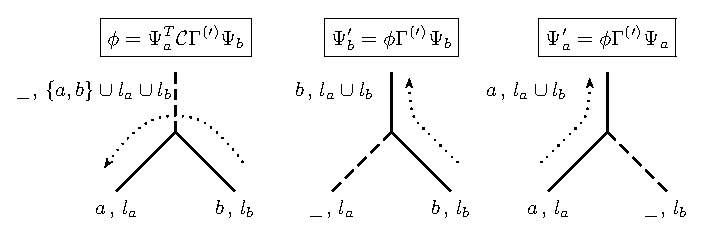
\includegraphics[width=.56\paperwidth]{fusion_rules}
\end{equation}
Here, $a$ and $b$ are the labels for the fermion from the left or
right leg, respectively. $l_a$ and $l_b$ are the closed fermions lines
contained in the 1POWs from the left and right leg,
respectively. Because the evaluation direction within O'Mega always
goes from right to left, a fermion pair in a fusion is always
collected as a pair $(a,b)$. The
\begin{figure}
\[  
\setlength{\extrarowheight}{2pt}    
\begin{array}{|c|c|}\hline
        {\bf \Gamma} & {\bf \Gamma'} \\\hline\hline     
        \parbox{13mm}{\hfil\\
        \begin{fmfgraph*}(12,10)
          \fmftop{t}
          \fmfbottom{b1,b2}
          \fmf{fermion}{v,b1}   \fmf{fermion}{b2,v}
          \fmf{dashes}{v,t}       
        \end{fmfgraph*}} \quad 
        \parbox{13mm}{\hfil\\
        \begin{fmfgraph*}(12,10)
          \fmftop{t}
          \fmfbottom{b1,b2}
          \fmf{plain}{v,b1}     \fmf{fermion}{b2,v}
          \fmf{dashes}{v,t}       
        \end{fmfgraph*}} \quad 
        \parbox{13mm}{\hfil\\
        \begin{fmfgraph*}(12,10)
          \fmftop{t}
          \fmfbottom{b1,b2}
          \fmf{plain}{v,b2}     \fmf{fermion}{v,b1}
          \fmf{dashes}{v,t}       
        \end{fmfgraph*}}        
 & 
        \parbox{13mm}{\hfil\\
        \begin{fmfgraph*}(12,10)
          \fmftop{t}
          \fmfbottom{b1,b2}
          \fmf{fermion}{b1,v}   \fmf{fermion}{v,b2}
          \fmf{dashes}{v,t}       
        \end{fmfgraph*}} \quad 
        \parbox{13mm}{\hfil\\
        \begin{fmfgraph*}(12,10)
          \fmftop{t}
          \fmfbottom{b1,b2}
          \fmf{plain}{v,b1}     \fmf{fermion}{v,b2}
          \fmf{dashes}{v,t}       
        \end{fmfgraph*}} \quad 
        \parbox{13mm}{\hfil\\
        \begin{fmfgraph*}(12,10)
          \fmftop{t}
          \fmfbottom{b1,b2}
          \fmf{plain}{v,b2}     \fmf{fermion}{b1,v}
          \fmf{dashes}{v,t}       
        \end{fmfgraph*}} 
\\ & \\
        \parbox{13mm}{\hfil\\
        \begin{fmfgraph*}(12,10)
          \fmftop{t}
          \fmfbottom{b2,b1}
          \fmf{plain}{v,b1}     \fmf{plain}{b2,v}
          \fmf{dashes}{v,t}       
        \end{fmfgraph*}} \quad 
        \parbox{13mm}{\hfil\\
        \begin{fmfgraph*}(12,10)
          \fmftop{t}
          \fmfbottom{b2,b1}
          \fmf{fermion}{b1,v}   \fmf{fermion}{b2,v}
          \fmf{dashes}{v,t}       
        \end{fmfgraph*}} 
  &
        \parbox{13mm}{\hfil\\
        \begin{fmfgraph*}(12,10)
          \fmftop{t}
          \fmfbottom{b2,b1}
          \fmf{fermion}{v,b2}   \fmf{fermion}{v,b1}
          \fmf{dashes}{v,t}       
        \end{fmfgraph*}} 
         \\ & \\\hline 
        \underline{\;\;} \, , \, \left\{ a , b \right\} \cup l_a \cup l_b & 
        \underline{\;\;} \, , \, \left\{ a , b \right\} \cup l_a \cup
        l_b \\\hline\hline \vspace{1pt}
        \parbox{13mm}{\hfil\\\hfil\\
        \begin{fmfgraph*}(12,10)
          \fmftop{t}
          \fmfbottom{b2,b1}
          \fmf{plain}{v,t}      \fmf{fermion}{b2,v}
          \fmf{dashes}{b1,v}      
        \end{fmfgraph*}} \quad 
        \parbox{13mm}{\hfil\\\hfil\\
        \begin{fmfgraph*}(12,10)
          \fmftop{t}
          \fmfbottom{b2,b1}
          \fmf{plain}{v,b2}     \fmf{fermion}{v,t}
          \fmf{dashes}{b1,v}      
        \end{fmfgraph*}} \quad
 & 
        \parbox{13mm}{\hfil\\\hfil\\
        \begin{fmfgraph*}(12,10)
          \fmftop{t}
          \fmfbottom{b2,b1}
          \fmf{fermion}{t,v}    \fmf{fermion}{v,b2}
          \fmf{dashes}{b1,v}      
        \end{fmfgraph*}} \quad 
                \parbox{13mm}{\hfil\\\hfil\\
        \begin{fmfgraph*}(12,10)
          \fmftop{t}
          \fmfbottom{b2,b1}
          \fmf{plain}{v,t}      \fmf{fermion}{v,b2}
          \fmf{dashes}{b1,v}      
        \end{fmfgraph*}} \quad 
        \parbox{13mm}{\hfil\\\hfil\\
        \begin{fmfgraph*}(12,10)
          \fmftop{t}
          \fmfbottom{b2,b1}
          \fmf{plain}{b2,v}     \fmf{fermion}{t,v}
          \fmf{dashes}{b1,v}      
        \end{fmfgraph*}}
         \\ & \\ 
        \parbox{13mm}{\hfil\\
        \begin{fmfgraph*}(12,10)
          \fmftop{t}
          \fmfbottom{b2,b1}
          \fmf{fermion}{b2,v}   \fmf{fermion}{t,v}
          \fmf{dashes}{b1,v}      
        \end{fmfgraph*}} 
        \quad
        \parbox{13mm}{\hfil\\
        \begin{fmfgraph*}(12,10)
          \fmftop{t}
          \fmfbottom{b2,b1}
          \fmf{plain}{b2,v}     \fmf{plain}{v,t}
          \fmf{dashes}{b1,v}      
        \end{fmfgraph*}}
        & 
        \parbox{13mm}{\hfil\\
        \begin{fmfgraph*}(12,10)
          \fmftop{t}
          \fmfbottom{b2,b1}
          \fmf{fermion}{v,t}    \fmf{fermion}{v,b2}
          \fmf{dashes}{b1,v}      
        \end{fmfgraph*}}        
        \\ & \\\hline 
        a \, , \,  l_a \cup l_b  & a \, , \,  l_a \cup l_b \\\hline
   \end{array}
\]
\caption{\label{fig:fusionmaj} 
Fusion rules for fermions with fermion-number violating interactions. 
For the fusions where a fermion is produced, there
are also mirror diagrams. $a, b$ are the labels
for the left fermion and the right fermion, respectively, and $l_a$ 
and $l_b$ are the corresponding closed fermion lines contained in the
subamplitudes. For the conventions concerning the fusions with
clashing arrows and with two Majorana fermions cf.~the text.}  
\end{figure}
box on top of the graph shows the analytical expression that is to be
calculated by O'Mega. $\Gamma$ is the gamma matrix expression at the
vertex, while $\Gamma'$ according to~\ref{eq:gammagammastrich} is the
charge-conjugated vertex expression that has to be inserted whenever
the evaluation direction is opposite to the fermion flow at the
corresponding line. As the canonical evaluation directions in O'Mega
are from bottom to top for open lines in fusions and from right to
left in lines being closed at fusions, Fig.~\ref{fig:fusionmaj}
collects all cases where the vertex expression is unchanged ($\Gamma$)
and where is has to be charge-conjugated ($\Gamma'$). Part of the
fermi statistics signs for fermion-number violating vertices is
encoded in these disentanglements, as explained
in~\cite{Denner:1992vza}. As the fermion lines for fermion-number
violating vertices are labeled not by pairs 
\verb+(conjugated external spinor, external spinor)+ but simply by 
\verb+(endpoint, starting point)+ for the evaluation direction for
fermion lines, the remaining 
sign factor for an amplitude can be calculated now again (as in the
case for purely fermion-number conserving interactions) by determining
the number of transpositions needed to bring the entries in the pair
to a canonical reference order. Note that a change of evaluation
direction for a single line would transform the pair $(a,b)$ into
$(b,a)$ resulting in an additional sign with respect to the reference
order. This is exactly the sign from an additional anticommutation of
Fermi field operators in Eq.~\ref{eq:entangle} and is recovered in the
relative sign between left and right hand side of
Eq.~\ref{eq:entangle2} coming from the antisymmetry of the
charge-conjugation matrix. 

The additional signs are encoded in the vertex factors. So, in the two
cases, when (i) sandwiching the vertex factor the left- and
right-handed spinorial expressions in the closing of a line or (ii) the
left-multiplication of the spinorial expression by the vertex factor
when continuing an open fermion line in a fusion from the bottom to
the top, there could appear additional signs. Namely, when the
evaluation directions as shown in Fig.~\ref{fig:fusionmaj} point
opposite to the (first) fermion arrow at the vertex there is a sign
change in the case of vectorial and tensorial couplings. For the
vertices in the first lines of the boxes in Fig.~\ref{fig:fusionmaj}
it is clear how to define the vertices and how to implement them into
O'Mega. Care, however, has to be taken in the case of the vertices in
the second lines, containg either clashing arrows or two Majorana
fermions. In the case of clashing arrows, we adopt the convention to
define vertices in the {\em O'Mega} model files having the
charge-conjugated particle on the left-hand side, i.e. define the
vertex as $\overline{\Psi^c_1} \Gamma \Psi_2$ instead of
$\overline{\Psi_1} \Gamma \Psi_2^c$; if we had defined them the other
way round, the diagrams with clashing arrows would have to be
exchanged between the two columns in Fig.~\ref{eq:fusionmaj}, as
evaluation direction would point then the other way round for these
vertices. For vertices with one Majorana and one Dirac line (e.g. the
electron--selectron--neutralino vertex) there are no ambiguities,
because the Dirac fermion automatically provides a unique
direction. The case for vertices with two Majorana fermions is more
complicated: If the two Majorana fermions are identical, the coupling
has to be scalar, pseudoscalar or axial-vectorial, hence there is no
issue with signs and ordering conventions. Consider now the case where
the Majorana fermions are indeed different, e.g. in the vertex of two
different MSSM neutralinos and the $Z$ boson. Here one has to decide
whether to define the vertex in the Lagrangian as
\begin{equation*}
        \overline{\tilde{\chi}^0_i} \left( g_V + g_A \gamma^5 \right)
        \fmslash{Z} \tilde{\chi}^0_j \qquad \text{or} \qquad
        \overline{\tilde{\chi}^0_j} \left( - g_V + g_A \gamma^5 \right)
        \fmslash{Z} \tilde{\chi}^0_i \;\; , \quad i \neq j \;\;,
\end{equation*}    
as well as in the model file. By adopting one of the two options, one
arbitrarily assigns a fermion arrow to the vertex:
\begin{equation*}
        \parbox{18mm}{\hfil\\\hfil\\
        \begin{fmfgraph*}(17,15)
          \fmfleft{l1,l2}
          \fmfright{r}
          \fmfbottom{b}
          \fmf{fermion,label=$\tilde{\chi}^0_j$,l.side=left}{l1,v}      
          \fmf{fermion,label=$\overline{\tilde{\chi}^0_i}$,l.side=right}{v,l2}
          \fmf{photon}{v,r}     
          \fmfdot{v}
          \fmflabel{$\boxed{\overline{\tilde{\chi}^0_i} \left( g_V + g_A
                        \gamma^5 \right) \fmslash{Z} \tilde{\chi}^0_j}$}{b}
        \end{fmfgraph*}\hfil\\\hfil\\} \qquad \qquad    \qquad \qquad 
        \parbox{18mm}{\hfil\\\hfil\\
        \begin{fmfgraph*}(17,15)
          \fmfleft{l1,l2}
          \fmfright{r}
          \fmfbottom{b}
          \fmf{fermion,label=$\tilde{\chi}^0_i$,l.side=left}{l1,v}      
          \fmf{fermion,label=$\overline{\tilde{\chi}^0_j}$,l.side=right}{v,l2}
          \fmf{photon}{v,r}
          \fmfdot{v}
          \fmflabel{$\boxed{\overline{\tilde{\chi}^0_j} \left( - g_V + g_A
                        \gamma^5 \right) \fmslash{Z} \tilde{\chi}^0_i}$}{b}
        \end{fmfgraph*}\hfil\\\hfil\\}
\end{equation*}
That pseudo-assignment of arrows means that when contracting the field
operators of that interaction vertex with external states or other
interaction vertices, then we had to write down a conjugated spinor
for the neutralino $i$ and a spinor for the neutralino $j$ on the left
hand side, and vice versa for the right hand side. In
Fig.~\ref{fig:fusionmaj} it is assumed that the vertex for two  
Majorana fermions is always defined within the O'Mega model files in
such a way that in the fusion process of two fermions the left one is
the conjugated spinor while in the case of the fermion line 
being continued, the fermion on top (i.e. the one fused to from the
children) is the conjugated. Henceforth no primed vertex factors have
to be used for vertices with two Majorana fermions. (In 
practice, there is a unique representation in O'Mega for such
vertices, so when the fusion does not match that
representation, then there {\em do} appear signs in front of the
vertex factors. E.g.~when we denote that neutralino neutral current by
the left possiblity above, but the second neutralino appears as a left leg
at a fusion and the first as a right leg, then the vector coupling
constant has to be endowed with an explicit extra minus sign).

After having discussed signs from vertex factors, we have to account
for possible signs from propagators for the implementation with
fermion-number violating vertices. In O'Mega, the momentum flow is
always outgoing, i.e. from the inside of an amplitude
outwards. Because the subamplitudes joined together in fusions are
made up from external states with outgoing momenta, momentum flow in
fusions is always from top to bottom (for all vertices):   
\begin{equation}
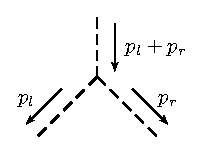
\includegraphics[width=.16\paperwidth]{mom_flow}
\end{equation}
After a fusion has taken place, a fermionic wavefunction (if it is not
already an external wavefunction e.g. in a decay amplitudes) is
multiplied by a propagator. Thus, every wavefunction 
appearing as a child (left or right leg) in a fusion is either a
wavefunction of an external fermion or has already been multiplied by a
propagator. An exception occurs if the wavefunction is the final
keystone of a subamplitude; then to only one of the fermionic
wavefunctions the propagator has to be assigned. Hence, a propagator is
inserted in all fusion cases where the fermion line is not closed but
runs through to the top. 

It turns out that only one type of propagator is need when handling 
both Dirac and Majorana fermions. The prescription
in~\ref{eq:propprime} shows that whenever the evaluation direction is
opposite to the arrow of a Dirac line, one has to use the primed
propagator, which means to revert the sign of the momentum within the
propagator. Of course, a momentum flow opposite to the fermion arrow
has the same effect. Collecting signs for fermion propagators yields:
\begin{equation}
        \parbox{18mm}{\hfil\\\hfil\\
        \begin{fmfgraph*}(17,9)
          \fmfleft{l}
          \fmfright{r}
          \fmfbottomn{b}{9}
          \fmftopn{t}{9}
          \fmf{fermion}{l,r}
          \fmf{dashes}{b3,b7}
          \fmf{dots}{t3,t7}
          \fmf{phantom_arrow}{b3,b2}    \fmf{phantom_arrow}{b7,b8}
          \fmf{phantom_arrow}{t3,t2}    \fmf{phantom_arrow}{t7,t8}
          \fmflabel{$p$}{b5}
        \end{fmfgraph*}\hfil\\} \quad =
        \dfrac{\ii}{\xi \fmslash{p} - m}, \qquad\qquad
        \parbox{18mm}{\hfil\\\hfil\\
        \begin{fmfgraph*}(17,9)
          \fmfleft{l}
          \fmfright{r}
          \fmfbottomn{b}{9}
          \fmftopn{t}{9}
          \fmf{plain}{l,r}
          \fmf{dashes}{b3,b7}
          \fmf{dots}{t3,t7}
          \fmf{phantom_arrow}{b3,b2}    \fmf{phantom_arrow}{b7,b8}
          \fmf{phantom_arrow}{t3,t2}    \fmf{phantom_arrow}{t7,t8}
          \fmflabel{$p$}{b5}
        \end{fmfgraph*}\hfil\\} \quad =
        \dfrac{\ii}{\zeta \fmslash{p} - m}
\end{equation}
where the sign factor $\xi$ is $+1$ if the
evaluation direction and the momentum flow are both parallel or
both antiparallel to the fermion arrow, and $-1$ otherwise. For
Majorana fermions, $\zeta$ is $+1$ if evaluation direction and
momentum flow coincide, and $-1$ otherwise. The
following table proofs that this in all cases leads to a negative sign
for the propagator momentum within O'Mega:

\begin{center}
\begin{tabular}{|l|c|c|c|c|}\hline
  fermion type & fermion arrow & mom. & eval. & sign \\\hline\hline
  Dirac fermion &     $\uparrow$  &  $\downarrow$ &
    $\uparrow$ & negative \\\hline
  Dirac antifermion & $\downarrow$ & $\downarrow$ &
    $\uparrow$ & negative   \\\hline
  Majorana fermion  & - & $\downarrow$ & $\uparrow$ & negative \\\hline
\end{tabular}
\end{center}                 
So the universally used fermion propagator for all types of fermions --
fermions, antifermions and Majorana fermions -- is
\begin{equation}
        \boxed{ S_{F,\text{\em O'Mega}} = \dfrac{\ii}{- \fmslash{p} -
        m} } 
\end{equation}

Finally, we are able to proof our conjecture that is always correct to
use the charge-conjuagated spinor in the bilinear product $\Psi^T_1
\mathcal{C} \Gamma \Psi_2$, even if the spinor expression from the
left leg of the fusion consists of a product of vertex and propagator
factors. Let
\begin{equation}
        \label{eq:leftleg}
        \Psi = S_F^{(1)} \Gamma^{(1)} S_F^{(2)} \ldots \Gamma^{(n)}
        w  , \qquad w \in \left\{ u, v \right\} \, . 
\end{equation}
be the spinor for the left leg as calculated by O'Mega just before it
is fused. When performing the fusion, O'Mega uses the expression
$\Psi^T \mathcal{C}$ for the left leg spinor in the product.
Inserting~Eq. (\ref{eq:leftleg}) gives:    
is equal to 
\begin{align}
        \Psi^T \mathcal{C} =&\; w^T  {\Gamma^{(n)}}^T
        \ldots {S_F^{(2)}}^T {\Gamma^{(1)}}^T {S_F^{(1)}}^T \left( -
        \mathcal{C}^{-1} \right)  \notag \\ =&\; 
        w^T  \left( - \mathcal{C} \right)
        \mathcal{C} {\Gamma^{(n)}}^T \mathcal{C}^{-1}
        \ldots \mathcal{C}  {S_F^{(2)}}^T \mathcal{C}^{-1} \mathcal{C}
         {\Gamma^{(1)}}^T \mathcal{C}^{-1}\mathcal{C}{S_F^{(1)}}^T \left( -
        \mathcal{C}^{-1} \right) \notag \\ 
        =&\; \overline{w^c} \, {\Gamma^{(n)}}' \ldots {S_F^{(2)}}' 
         {\Gamma^{(1)}}' {S_F^{(1)}}' 
         \label{eq:finalreverse}
\end{align}
We have already explained that the assignment of the wavefunction for
the external fermion is correct. Now we get the primed expressions for
all vertex factors and propagators. But that is what we want,
since, indeed, our evaluation direction for the whole fermion 
line -- after the fermion line has been closed by the fusion -- 
has been reverted. This closes the proof of the correctness of the
implementation of the algorithm for fermion-number violating
vertices. 


\subsection{Cross checks and tests}

The implementation of the formalism for models with fermion-number
violating vertices has been extensively tested and verified. First of
all, the algorithm and its implementation outlined above can also be
applied to models with fermion number conservation in all vertices,
which include QED, QCD, and the Standard Model. It has been verified
that using the algorithm described in part I~\cite{Moretti:2001zz} and
the one here yield numerically identical results. The methods
described here have been successfully used to construct and test Ward
and Slavnov-Taylor identities in supersymmetric gauge field
theories~\cite{Ohl:2002jp}. All cross checks of O'Mega and
WHIZARD~\cite{Kilian:2007gr} with other codes for models containing
fermion-number violating interactions, e.g. in the MSSM and the
NMSSM~\cite{Hagiwara:2005wg,Reuter:2009ex}, have proved the validity
of the algorithm and its implementation. A very stringent and
extensive test has been performed in the procedure of validating the
interface of WHIZARD and O'Mega to the program
FeynRules~\cite{Christensen:2010wz}. 

%%%%%%%%%%%%%%%%%%%%%%%%%%%%%%%%%%%%%%%%%%%%%%%%%%%%%%%%%%%%%%%%%%%%%%%%
\section*{Acknowledgements}

Special thanks go to the \OMEGA/ contributors,
F.~Bach, F.~Braam, and especially C.~Speckner. Furthermore, we would
like to thank A.~Alboteanu, E.~Boos, P.~Manakos, M.~Moretti,
D.~Ondreka, H.~Reuter, and C.~Schwinn for valuable discussions,
comments and help during this project. WK and JR acknowledge the
friendly atmosphere within and support by the 
particle physics groups at the University of Karlsruhe and DESY,
Hamburg, and the Aspen Center for Physics, where a lot of this work
has been initiated. JR wants especially to thank the particle physics
group at Carleton University, Ottawa, where part of this work has been
completed, for their warm hospitality and lots of interesting
discussions.  WK expresses his particular gratitude for the warm
hospitality and support of the particle physics group at the
University of Urbana/Champaign.  We would like to extend particular
gratitude to C.~Schwinn for his work on $R_\xi$-gauge functors and
tests of gauge parameter independence in \OMEGA/ amplitudes, and also
for many helpful and enlightening discussions in an early stage of
\OMEGA/.

This work has been supported in part by the Helmholtz-Gemeinschaft
under Grant No.{} VH-NG-005, the Helmholtz alliance ``Physics at the
Terascale'', the Bundesministerium f\"ur Bildung und
For\-schung, Germany, (Grant No. 05\,HT9RDA, 05 HA6VFB, 05\,H4WWA/2,
05\,H09PSE), the Ministerium f\"ur Wissenschaft und Kultur of the
state Baden-W\"urttemberg, and the Deut\-sche
For\-schungs\-ge\-mein\-schaft (single projects MA\,676/6-1 and RE
2850/1-1 as well as by the Graduier\-ten\-kolleg GK 1102 ``Physics at
Hadron Colliders''). 

%%%%%%%%%%%%%%%%%%%%%%%%%%%%%%%%%%%%%%%%%%%%%%%%%%%%%%%%%%%%%%%%%%%%%%%%
\begin{thebibliography}{10}

\bibitem{Moretti:2001zz}
  M.~Moretti, T.~Ohl, J.~Reuter,
  %``O'Mega: An optimizing matrix element generator,''
  [arXiv:hep-ph/0102195].
  %%CITATION = HEP-PH/0102195;%%

\bibitem{Kilian:2007gr}
  W.~Kilian, T.~Ohl, J.~Reuter,
  %``WHIZARD: Simulating Multi-Particle Processes at LHC and ILC,''
  Eur.{} Phys.{} J.{} \textbf{C71} (2011)  1742
  [arXiv:0708.4233 [hep-ph]].

\bibitem{Maltoni:2002mq}
  F.~Maltoni, K.~Paul, T.~Stelzer, S.~Willenbrock,
  %``Color flow decomposition of QCD amplitudes,''
  Phys.{} Rev.{}  \textbf{D67} (2003) 014026
  [hep-ph/0209271].

\bibitem{cflow}
 W.~Kilian, T.~Ohl, J.~Reuter, C.~Speckner,
 \textit{QCD in the Color-Flow Representation},
 in preparation.

\bibitem{Haber:1984rc}
  H.~E.~Haber, G.~L.~Kane,
  %``The Search for Supersymmetry: Probing Physics Beyond the Standard Model,''
  Phys.\ Rept.\  {\bf 117}, 75-263 (1985).
  
\bibitem{Denner:1992vza}
  A.~Denner, H.~Eck, O.~Hahn, J.~Kublbeck,
  %``Feynman rules for fermion number violating interactions,''
  Nucl.\ Phys.\  {\bf B387}, 467-484 (1992).

\bibitem{Reuter:2002gn}
  J.~Reuter,
  \textit{Supersymmetry of scattering amplitudes and Green functions
    in perturbation theory},
  PhD Thesis, Darmstadt University of Technology, 2002
  [arXiv:hep-th/0212154].
  %%CITATION = HEP-TH/0212154;%%

\bibitem{Ohl:2002jp}
  T.~Ohl, J.~Reuter,
  %``Clockwork SUSY: Supersymmetric Ward and Slavnov-Taylor identities at work
  %in Green's functions and scattering amplitudes,''
  Eur.\ Phys.\ J.\  C {\bf 30}, 525 (2003)
  [arXiv:hep-th/0212224].
  %%CITATION = EPHJA,C30,525;%%

\bibitem{Hagiwara:2005wg}
  K.~Hagiwara, W.~Kilian, F.~Krauss, T.~Ohl, T.~Plehn, D.~Rainwater, J.~Reuter, S.~Schumann,
  %``Supersymmetry simulations with off-shell effects for CERN LHC and ILC,''
  Phys.\ Rev.\  {\bf D73}, 055005 (2006).
  [hep-ph/0512260].

\bibitem{Reuter:2009ex}
  J.~Reuter, F.~Braam,
  %``The NMSSM implementation in WHIZARD,''
  AIP Conf.\ Proc.\  {\bf 1200}, 470-473 (2010).
  [arXiv:0909.3059 [hep-ph]].

\bibitem{Christensen:2010wz}
  N.~D.~Christensen, C.~Duhr, B.~Fuks, J.~Reuter, C.~Speckner,
  %``Exploring the golden channel for HEIDI models using an interface between WHIZARD and FeynRules,''  
  [arXiv:1010.3251 [hep-ph]].


%\cite{Hagiwara:2010vk}
\bibitem{Hagiwara:2010vk}
  K.~Hagiwara, Y.~Takaesu,
  %``Generating QCD amplitudes in the color-flow basis with MadGraph,''
  Eur.\ Phys.\ J.\  {\bf C71 } (2011)  1668.
  [arXiv:1010.0748 [hep-ph]].

\bibitem{Kleiss:2009pm}
  R.~Kleiss and G.~van den Oord,
  %``Recursive equations for Majorana currents,''
  arXiv:0906.0697 [hep-ph].
  %%CITATION = ARXIV:0906.0697;%%

\end{thebibliography}

%%%%%%%%%%%%%%%%%%%%%%%%%%%%%%%%%%%%%%%%%%%%%%%%%%%%%%%%%%%%%%%%%%%%%%%%
\end{empfile}
\end{fmffile}
\end{document}
\endinput
Local Variables:
mode:latex
indent-tabs-mode:nil
page-delimiter:"^%%%%%.*\n"
End:

